\documentclass[a4paper,12pt,titlepage]{article}
\usepackage{graphicx}
\usepackage[hidelinks]{hyperref}
\usepackage{listings}
\usepackage{float}
\DeclareGraphicsExtensions{.bmp,.eps,.jpg,.png}

\begin{document}
%\title and intnro
\begin{titlepage}
	\begin{center}
		
		\begin{figure}[t]
			\centering
			
\includegraphics[width=450px]{./Graphics/KPTH_Logo}
		\end{figure}		
		
		\textbf{\LARGE Gynaecological Patient Information
		Management System:}
		
		\vspace{1 cm}
	    \textbf{\LARGE \\Software Test Documentation}
		
		\vspace{1 cm}
		\LARGE{\textbf{Team Pentec: }}
		

		\begin{flushright} \large
			
			Ruth Ojo 12042804\newline
			Liz Joseph 10075268\newline
			Trevor Austin 11310856\newline
			Maria Qumayo 29461775\newline
			Lindelo Mapumulo 12002862\newline
		\end{flushright}
		
				\vspace{1 cm}
				\centering
				
\includegraphics[width=150px]{./Graphics/Pentec_Logo.png}

		
		
		{\LARGE Final Version}
		\\
		{\large \today}		
		
		
	\end{center}
\end{titlepage}

%\table of content
\tableofcontents
\newpage

\section{Introduction}
%\Intro
\section{Introduction}

This document documents and taracks the necessary information required to effectively define the approach to be used in the testing and evaluationg of the Patient Information Management System designed by the group Pentect for the Kalafong 

The following Patient Infromation Management System Use cases that were thoroughly tested are:

\begin{itemize}
	\item User Login
	\item PIMS Artificial Intelligence
	\item PIMS Statistics
	\item PIMS Notifications
	\item PIMS Space
\end{itemize}

Testing was done on the system mainly for the following 5 reasons:

\begin{itemize}
	\item To ensure that the system meets both functional and non functional requirements arroding to the given spesifications
	\item System stress. To make sure that the system does not fail with multiple users
	\item To handle and resolve with System failures and bugs appropriatly and in good time.
	\item PIMS Notifications
	\item To ensure that the final product is of top, professiona, software engineering standards.
\end{itemize}


\newpage	
\section{Features and Items tested}
%By Maria
\subsection{Features and Items tested}

Our testing involved looking at the core functional requirements as given in our client's spesification document. As well as those we added on as "Nice to have". The following use cases and features as depicted in the PIMS master Node Scope were tested.
\newline

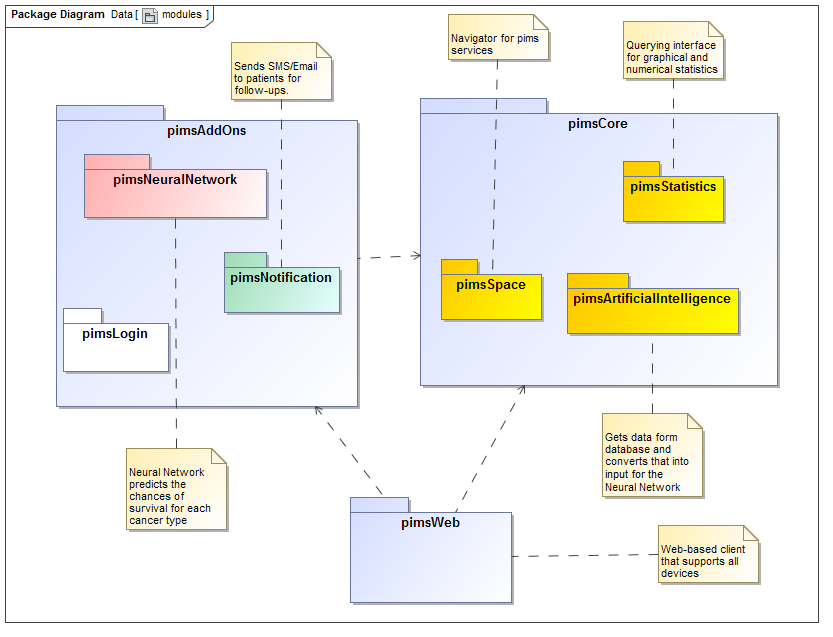
\includegraphics[width=\linewidth]{./Graphics/modules.png}
\newline

		Functional Testing
		- for each use case tested
		* either success or a list of violations of the contract requirements
		* a test coverage analysis reporting which percentage of the use cases have been covered by the testing
		
		2. Non-functional testing/assessment
		- any performance, scalability, maintainability, reliability, usability,security, maintainability problems identified with evidence for the identified problem.
	
\newpage			

\section{Functional Testing}
	\subsection{PIMS Login}
	%By Maria/
 \subsubsection{Pims Login}
Pims User login testes for correct authentication and identification before the user is allowed system access. Further testing was done for user rights and privilages.
\newline

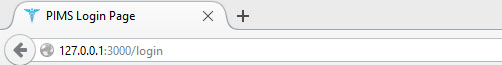
\includegraphics[width=\linewidth]{./Graphics/login.jpg}
\newline

Front end representation
\newline

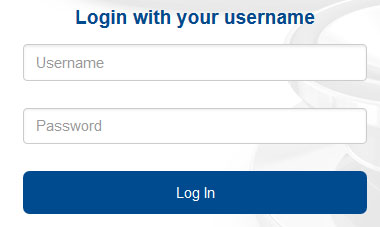
\includegraphics[width=\linewidth]{./Graphics/frontEnd.jpg}
		
User Authentication tested for the following conditions					
	\begin{itemize}
				\item Provide user with access
				\item Retrieve username
				\item Retrieve user password
				\item Fail with empty username and/ or empty password
				\item Return a boolean with regards to user right.
 \end{itemize}
 
 The figure bellow depics the successful testing of the Authentication and checkAdmin functions.
 \newline
 
 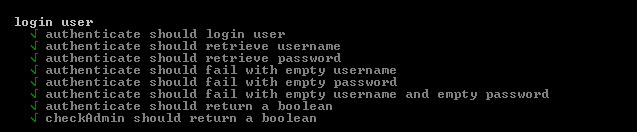
\includegraphics[width=\linewidth]{./Graphics/userResults.jpg}
 
 \subsubsection{Remarks}
 	\begin{itemize}
 				\item Pre-Conditions
 		User does not have access to systme.
 				\item Post-Conditions
 With correct login details, user successfuly gains access into the system with.
 User rights are checked upon login authentication
  \end{itemize}
  
  Both Pre and Post conditions  are considered in the implimentation of the system login. Unit testing successfuly.  tested with no violations to the security of the systm.
 
	
	\subsection{PIMS Notifications}
	%By Maria/
 \subsubsection{Pims Login}
Pims Send Notification is a two part function that we tested. First check if user is found(exists) in the database. Then send email using smtp.The unit test codes bellow demonstrates.
\newline

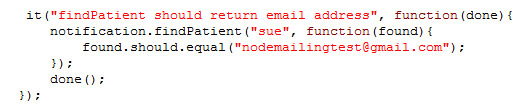
\includegraphics[width=\linewidth]{./Graphics/find.jpg}
\newline

Send Notifications via email
\newline

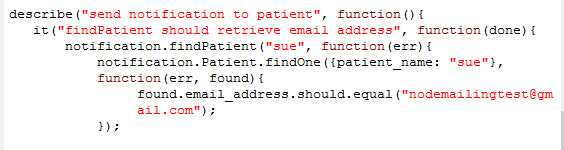
\includegraphics[width=\linewidth]{./Graphics/send.jpg}
The following conditions must be true for the send notification use case to pass.					
	\begin{itemize}
				\item Find patient should query the database to see if a user exists by searching for an email adress.
				\item Oce user is found, send notification must send and email to the found adress.
 \end{itemize}
 
 The figure bellow depics the successful testing of the Send Notification and FindUser functions.
 \newline
 
 \includegraphics[width=\linewidth]{./Graphics/Notify.jpg}
 
 \subsubsection{Remarks}
 	\begin{itemize}
 				\item Pre-Conditions
 		User must exist in database and have and email.
 				\item Post-Conditions
	User recieves and email from Prof Snyman.
  \end{itemize}
  
  Both Pre and Post conditions  are considered in the implimentation of sending notifications. Unit testing successfuly.  tested with no violations to the security of the systm.
 
	
	\subsection{PIMS Edit Profile}
	%By Maria/
 \subsubsection{Pims Login}
Pims edit user profile should be able to allow the admin user to update his profile and edit his information accordingly.
\newline

The Code bellow demonstrates the update of the user name after retrienving it.
\newline
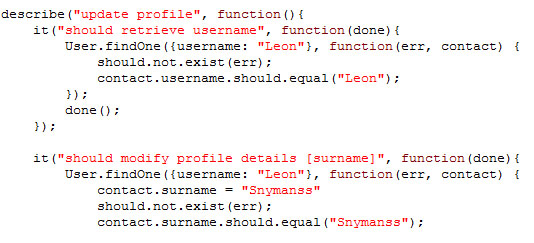
\includegraphics[width=\linewidth]{./Graphics/editCode.jpg}
\newline
		
Edit profile was  tested for the following conditions					
	\begin{itemize}
				\item Retrieve data
				\item Modify profile details
 \end{itemize}
 

 The figure bellow depics the successful testing of the UpdateAuthentication and checkAdmin functions.
 \newline
 
 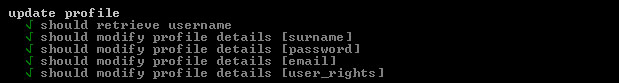
\includegraphics[width=\linewidth]{./Graphics/editProfile.jpg}

 
	
	\subsection{PIMS Add User}
	%\%By Maria
\subsection{Login and Admnistartive user}
	\subsubsection*{PIMS Login}
		Functional Testing
		- for each use case tested
		* either success or a list of violations of the contract requirements (pre- and post-condition violations or data structure requirements)
		* a test coverage analysis reporting which percentage of the use cases have been covered by the testing
		
		2. Non-functional testing/assessment
		- any performance, scalability, maintainability, reliability, usability, ... problems identified with evidence for the identified problem.
	
				
					\begin{itemize}
							\item The Buzz Space system has to accommodate and host a multitude of users concurrently, thus making it prone to various malfunctions and glitches
							
							\item The Space needs to be monitored in real time at all times to ensure relevance of topics and subject matters.
							\item The rating and tagging functionality need to be fair and accurate
							
							\item Sufficient feedback and updates of the Buzz Space state must be provided to the users. Users that create threads or just comment on one.
							
							\item General software control and application usage..
						 \end{itemize}
	
	\subsection{PIMS Artificial Inteligence}
%\	%By Maria
\subsection{Login and Admnistartive user}
	\subsubsection*{PIMS Login}
		Functional Testing
		- for each use case tested
		* either success or a list of violations of the contract requirements (pre- and post-condition violations or data structure requirements)
		* a test coverage analysis reporting which percentage of the use cases have been covered by the testing
		
		2. Non-functional testing/assessment
		- any performance, scalability, maintainability, reliability, usability, ... problems identified with evidence for the identified problem.
	
				
					\begin{itemize}
							\item The Buzz Space system has to accommodate and host a multitude of users concurrently, thus making it prone to various malfunctions and glitches
							
							\item The Space needs to be monitored in real time at all times to ensure relevance of topics and subject matters.
							\item The rating and tagging functionality need to be fair and accurate
							
							\item Sufficient feedback and updates of the Buzz Space state must be provided to the users. Users that create threads or just comment on one.
							
							\item General software control and application usage..
						 \end{itemize}
	
	\subsection{PIMS Statistics}
%\	%By Maria
\subsection{Login and Admnistartive user}
	\subsubsection*{PIMS Login}
		Functional Testing
		- for each use case tested
		* either success or a list of violations of the contract requirements (pre- and post-condition violations or data structure requirements)
		* a test coverage analysis reporting which percentage of the use cases have been covered by the testing
		
		2. Non-functional testing/assessment
		- any performance, scalability, maintainability, reliability, usability, ... problems identified with evidence for the identified problem.
	
				
					\begin{itemize}
							\item The Buzz Space system has to accommodate and host a multitude of users concurrently, thus making it prone to various malfunctions and glitches
							
							\item The Space needs to be monitored in real time at all times to ensure relevance of topics and subject matters.
							\item The rating and tagging functionality need to be fair and accurate
							
							\item Sufficient feedback and updates of the Buzz Space state must be provided to the users. Users that create threads or just comment on one.
							
							\item General software control and application usage..
						 \end{itemize}
	
	\subsection{PIMS Predictions}
%\	%By Maria/
 \subsubsection{Pims Login}
Pims User login testes for correct authentication and identification before the user is allowed system access. Further testing was done for user rights and privilages.
\newline

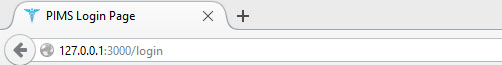
\includegraphics[width=\linewidth]{./Graphics/login.jpg}
\newline

Front end representation
\newline

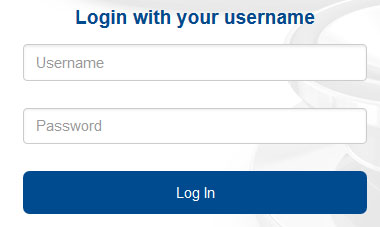
\includegraphics[width=\linewidth]{./Graphics/frontEnd.jpg}
		
User Authentication tested for the following conditions					
	\begin{itemize}
				\item Provide user with access
				\item Retrieve username
				\item Retrieve user password
				\item Fail with empty username and/ or empty password
				\item Return a boolean with regards to user right.
 \end{itemize}
 
 The figure bellow depics the successful testing of the Authentication and checkAdmin functions.
 \newline
 
 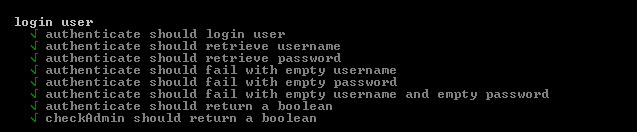
\includegraphics[width=\linewidth]{./Graphics/userResults.jpg}
 
 \subsubsection{Remarks}
 	\begin{itemize}
 				\item Pre-Conditions
 		User does not have access to systme.
 				\item Post-Conditions
 With correct login details, user successfuly gains access into the system with.
 User rights are checked upon login authentication
  \end{itemize}
  
  Both Pre and Post conditions  are considered in the implimentation of the system login. Unit testing successfuly.  tested with no violations to the security of the systm.
 
	
	
\section{Non-functional Testing}
	\subsection{Usability}
%\	%\subsection{Usability}
\subsubsection*{Description}
This ensures that a user will be able to use the system, with ease. The system should provide support to the user.
\subsubsection*{Justification}
The Patient information management system is user-oriented. How the users interact with the system is critical, and this should be done with little to no effort. The system should appear easy to use and should not, at any point, baffle the users. 
\subsubsection*{Mechanism}
	\begin{enumerate}
		\item Strategy:
		
		 \begin{itemize}
		 	\item A tutorial on how the patient information management system works. A user can be initiated into the system, the first time they use it. Or they can enable the tutorial until they're familiar with the functionality.
		 	\item Enable the user to troubleshoot their problems. Frequently asked questions or frequent problems could assist with this aspect.  A user will be provided with predefined help options such that they will not need to contact the system's administrator, for assistance.
		 	\item Provide descriptive headings that make navigation easier. Headings should not be ambiguous. A user should know what to expect when they select a certain heading.
		 	\item Error signals should be displayed to the user, if some user-inflicted error occurs. The necessary steps to rectify this problem must be provided.
		 	\item A user should be able to undo their action, should they be aware of their mistake.
		 \end{itemize}
		 	
		\item Architectural Pattern(s):
		
		\begin{itemize}
			\item Model-View-Controller: This separates the user interface from the rest of the system (Bass and John). A user should only interact with a simple interface that was designed for them. This is describable for patient information management system because the users don't necessary have an adept understanding of the lower   levels of the system.
		\end{itemize}
	\end{enumerate}
	
	\subsection{Scalability}
%\	\subsubsection*{Description}
The PIMS should be easily Maintainable in future. Thus needs to be flexible and extensible.
		
\subsubsection*{Justification}
Software always needs new features or bug fixes. Maintainable software is easy to extend and fix, which encourages the software's uptake and use.
	
	
\subsubsection*{Mechanism}	
\begin{enumerate}
\item Strategy:
	\begin{itemize}
		\item Open-source resources: using open source resources to minimize update costs in the future.
		\item Iterative development and regular reviews: This will help us improve system quality.
		\item Prevention is better than cure: Here we get others(lecturers) to review your code, to make sure its clean.The cleaner our code, the cheapre it is to maintain.
		\item Version control:Thsi will help keep our code, tests and documentation up to date and synchronised. It will also help us keep track of progress.
		\item Documentation: Relevant documentation will help future developers understand the software and system as a whole.
\end{itemize}
					
\end{enumerate}
	
	\subsection{Performance}
%\	\subsubsection*{Description}
The PIMS should be easily Maintainable in future. Thus needs to be flexible and extensible.
		
\subsubsection*{Justification}
Software always needs new features or bug fixes. Maintainable software is easy to extend and fix, which encourages the software's uptake and use.
	
	
\subsubsection*{Mechanism}	
\begin{enumerate}
\item Strategy:
	\begin{itemize}
		\item Open-source resources: using open source resources to minimize update costs in the future.
		\item Iterative development and regular reviews: This will help us improve system quality.
		\item Prevention is better than cure: Here we get others(lecturers) to review your code, to make sure its clean.The cleaner our code, the cheapre it is to maintain.
		\item Version control:Thsi will help keep our code, tests and documentation up to date and synchronised. It will also help us keep track of progress.
		\item Documentation: Relevant documentation will help future developers understand the software and system as a whole.
\end{itemize}
					
\end{enumerate}
	
	\subsection{Maintainability}
%\	\subsubsection*{Description}
The PIMS should be easily Maintainable in future. Thus needs to be flexible and extensible.
		
\subsubsection*{Justification}
Software always needs new features or bug fixes. Maintainable software is easy to extend and fix, which encourages the software's uptake and use.
	
	
\subsubsection*{Mechanism}	
\begin{enumerate}
\item Strategy:
	\begin{itemize}
		\item Open-source resources: using open source resources to minimize update costs in the future.
		\item Iterative development and regular reviews: This will help us improve system quality.
		\item Prevention is better than cure: Here we get others(lecturers) to review your code, to make sure its clean.The cleaner our code, the cheapre it is to maintain.
		\item Version control:Thsi will help keep our code, tests and documentation up to date and synchronised. It will also help us keep track of progress.
		\item Documentation: Relevant documentation will help future developers understand the software and system as a whole.
\end{itemize}
					
\end{enumerate}
	
	\subsection{Reliability}
%\	\subsection{Reliability and Availability}
\subsubsection*{Description}
The PIMS should be accessible at almost all times, in particular during the peak operational hours of the hospital. This accessibility will be limited to the hospital network only, so as to ensure no information can be changed without approval.
		
\subsubsection*{Justification}
The reliability and availability requirements are very important seeing as the information to be kept on the system is highly valuable to the medical staff, as the need up-to-date information concerning the patients they are dealing with (lives could be at risk).							 
With this in mind, only a downtime of less than 2 hours, at most twice a month will be allowed, so as too allow for the medical staff to maximally use the system.
A high reliability rate is recommended to ensure that users do not encounter any errors and/or data corruption in their use of the system. The only leeway that will be given for errors, is to have at most one.
	
	
\subsubsection*{Mechanism}	
\begin{enumerate}
\item Strategy:
	\begin{itemize}
		\item Clustering: using more resources by running many instances of the application over a cluster of servers or instances; therefore if any server should fail, the reliability and availability of the system will not be compromised.
		\item For reading from and writing to the database, we will ensure that no parallel updates are possible through enforcing the use of a single object to stream all database transactions; thus reducing inaccuracy that would be a result of data redundancy.		 
		\item Use of more resources: This would heavily reduce system downtime, as a temporary server can be run while the other is maintained.
\end{itemize}
					
\end{enumerate}

	
	\subsection{Secutity}
%\	\subsubsection*{Description}
The PIMS should be easily Maintainable in future. Thus needs to be flexible and extensible.
		
\subsubsection*{Justification}
Software always needs new features or bug fixes. Maintainable software is easy to extend and fix, which encourages the software's uptake and use.
	
	
\subsubsection*{Mechanism}	
\begin{enumerate}
\item Strategy:
	\begin{itemize}
		\item Open-source resources: using open source resources to minimize update costs in the future.
		\item Iterative development and regular reviews: This will help us improve system quality.
		\item Prevention is better than cure: Here we get others(lecturers) to review your code, to make sure its clean.The cleaner our code, the cheapre it is to maintain.
		\item Version control:Thsi will help keep our code, tests and documentation up to date and synchronised. It will also help us keep track of progress.
		\item Documentation: Relevant documentation will help future developers understand the software and system as a whole.
\end{itemize}
					
\end{enumerate}
	
	\subsection{Monitorability}
%\	%Monitorability
	\subsubsection*{Description}
		Audititabily or Monitor-ability is a software review where one or more auditors/monitors who are not members of the software development and organization team conduct "An independent examination of the software product to assess compliance with specifications, standards, contractual agreements, functional requirements and other criteria according to the development specification. Software Monitor-ability and audiability is different from testing or peer reviews because they are done by personnel external to and independent of the software development organization.
	\subsubsection*{Justification}
	Although it is important for the PIMS to be monitorable, it is not crucial. It may be Monitored because of the following:
					\begin{itemize}
							\item Multiple and concurrent users, thus making it prone to various malfunctions.
							
							\item Form filling and Statistical quering needs to be done in real time at all times to ensure relevance of topics and subject matters.
							
							\item Sufficient feedback and updates of the site's state must be provided to the users.
							
							\item General software control and application usage..
						 \end{itemize}
	
	\subsubsection*{Mechanism}
		\begin{enumerate}
			\item Strategy:\\\\
			Auditability and monitor-ability will be achieved by allowing any third party software auditor or monitor support group reviewing the Buzz Space examining it specifically for the aspects of the functional requirements as given by the client. Information such as the systems state and processes in complaints with the specification given. One such auditor may be from a well-established organisation, for example Oracle’s PeopleSoft enterprise which is UP’s current used application.	
			
			
			 \item Pattern/Tools:\\\\
			 Tools like SMaRT, a workbench for reporting the monitor-ability of Service Level Agreements for software services such as Buzz Space may be used. SMaRT aims to clearly identify the service level the service level commitments established between service requesters and providers. This monitoring infrastructure can be used with mechanical support groups in the form of a SMaRT Workbench Eclipse IDE plug-in for reporting on the monitor-ability of Service Level Agreements.
			 
		\end{enumerate}

	
\section{Remarks}
	\subsection{Risks and issues}
%\	\input{./Risks.tex}
	
	\subsection{Product quality}
%\	\subsubsection*{Description}
The PIMS should be easily Maintainable in future. Thus needs to be flexible and extensible.
		
\subsubsection*{Justification}
Software always needs new features or bug fixes. Maintainable software is easy to extend and fix, which encourages the software's uptake and use.
	
	
\subsubsection*{Mechanism}	
\begin{enumerate}
\item Strategy:
	\begin{itemize}
		\item Open-source resources: using open source resources to minimize update costs in the future.
		\item Iterative development and regular reviews: This will help us improve system quality.
		\item Prevention is better than cure: Here we get others(lecturers) to review your code, to make sure its clean.The cleaner our code, the cheapre it is to maintain.
		\item Version control:Thsi will help keep our code, tests and documentation up to date and synchronised. It will also help us keep track of progress.
		\item Documentation: Relevant documentation will help future developers understand the software and system as a whole.
\end{itemize}
					
\end{enumerate} 
	
	\subsection{Possible improvements}
%\	\input{./improvements.tex}

\section{Conclusion}
	

\end{document}